\begin{flushleft}
\doublespacing
\subsection{Sekvensdiagram}
Med fodfæste i analysediagrammerne har vi udarbejdet et sekvensdiagram, der illustrerer de overordnede funktioner, der bliver udført af systemer, når man ruller med en terning, rollDice(se figur 5.1.1). Her kaldes altså på metoden diceRoll hos Dice, hvorefter der bliver returneret terningernes øjne. Herefter kalder Game på getPosition hos Player, der returnerer den nuværende spillers position, hvorefter der udregnes en ny position. Når den nye position er fundet, kalder Game landOnField metoden hos Field, som er en abstrakt klasse - metoden er derfor polymorfisk. I følgende paragraffer beskrives hver polymorfisk case.Efter eksekvering af den landOnField tjekker Game for spillets regler hos Rules. Hvis en spiller har mindre en 0 stående på kontoen returnerer Rules en vinder. Herefter opdateres GUIen, hvor der til sidst skifter til næste spiller.
\addlinespace
For nedarvningen ChanceField (se figur 5.1.2) kalder ChanceField på drawChanceCard og executeChanceCard hos ChanceCard. Her trækkes altså et 'tilfældigt' kort, som eksekverer en handling. For at holde diagrammet simpelt viser vi ikke hvert chancekorts udførelse.
\addlinespace
For nedarvningen CustomField står en Player blot stille og der eksekveres altså ikke metoder (se figur 5.1.3).
\addlinespace
For nedarvningen JailField (se figur 5.1.4) kalder JailField på Player, som sætter Player i fængsel, isInJail = true. Hvis en Player ikke besidder et hasGetOutOfJailCard bliver der altså trukket penge fra Player's konto.
\addlinespace
For nedarvningen PropertyField (se figur 5.1.5) kaldes der på Account, setBalance, hvis feltet ikke allerede er købt - her købes feltet så og der trækkes prisen fra kontobalancen, Account. Hvis feltet er købt skal der betales leje, så der kaldes på setBalance hos Account med parametrene currentPlayer og owner, hvor der hhv. subtraheres og adderes med rent.
\addlinespace
I sidste nedarvning, StartField (se figur 5.1.6), kaldes på metoden addBalance hos Account, som tilfører currentPlayer 2 point til kontoen.
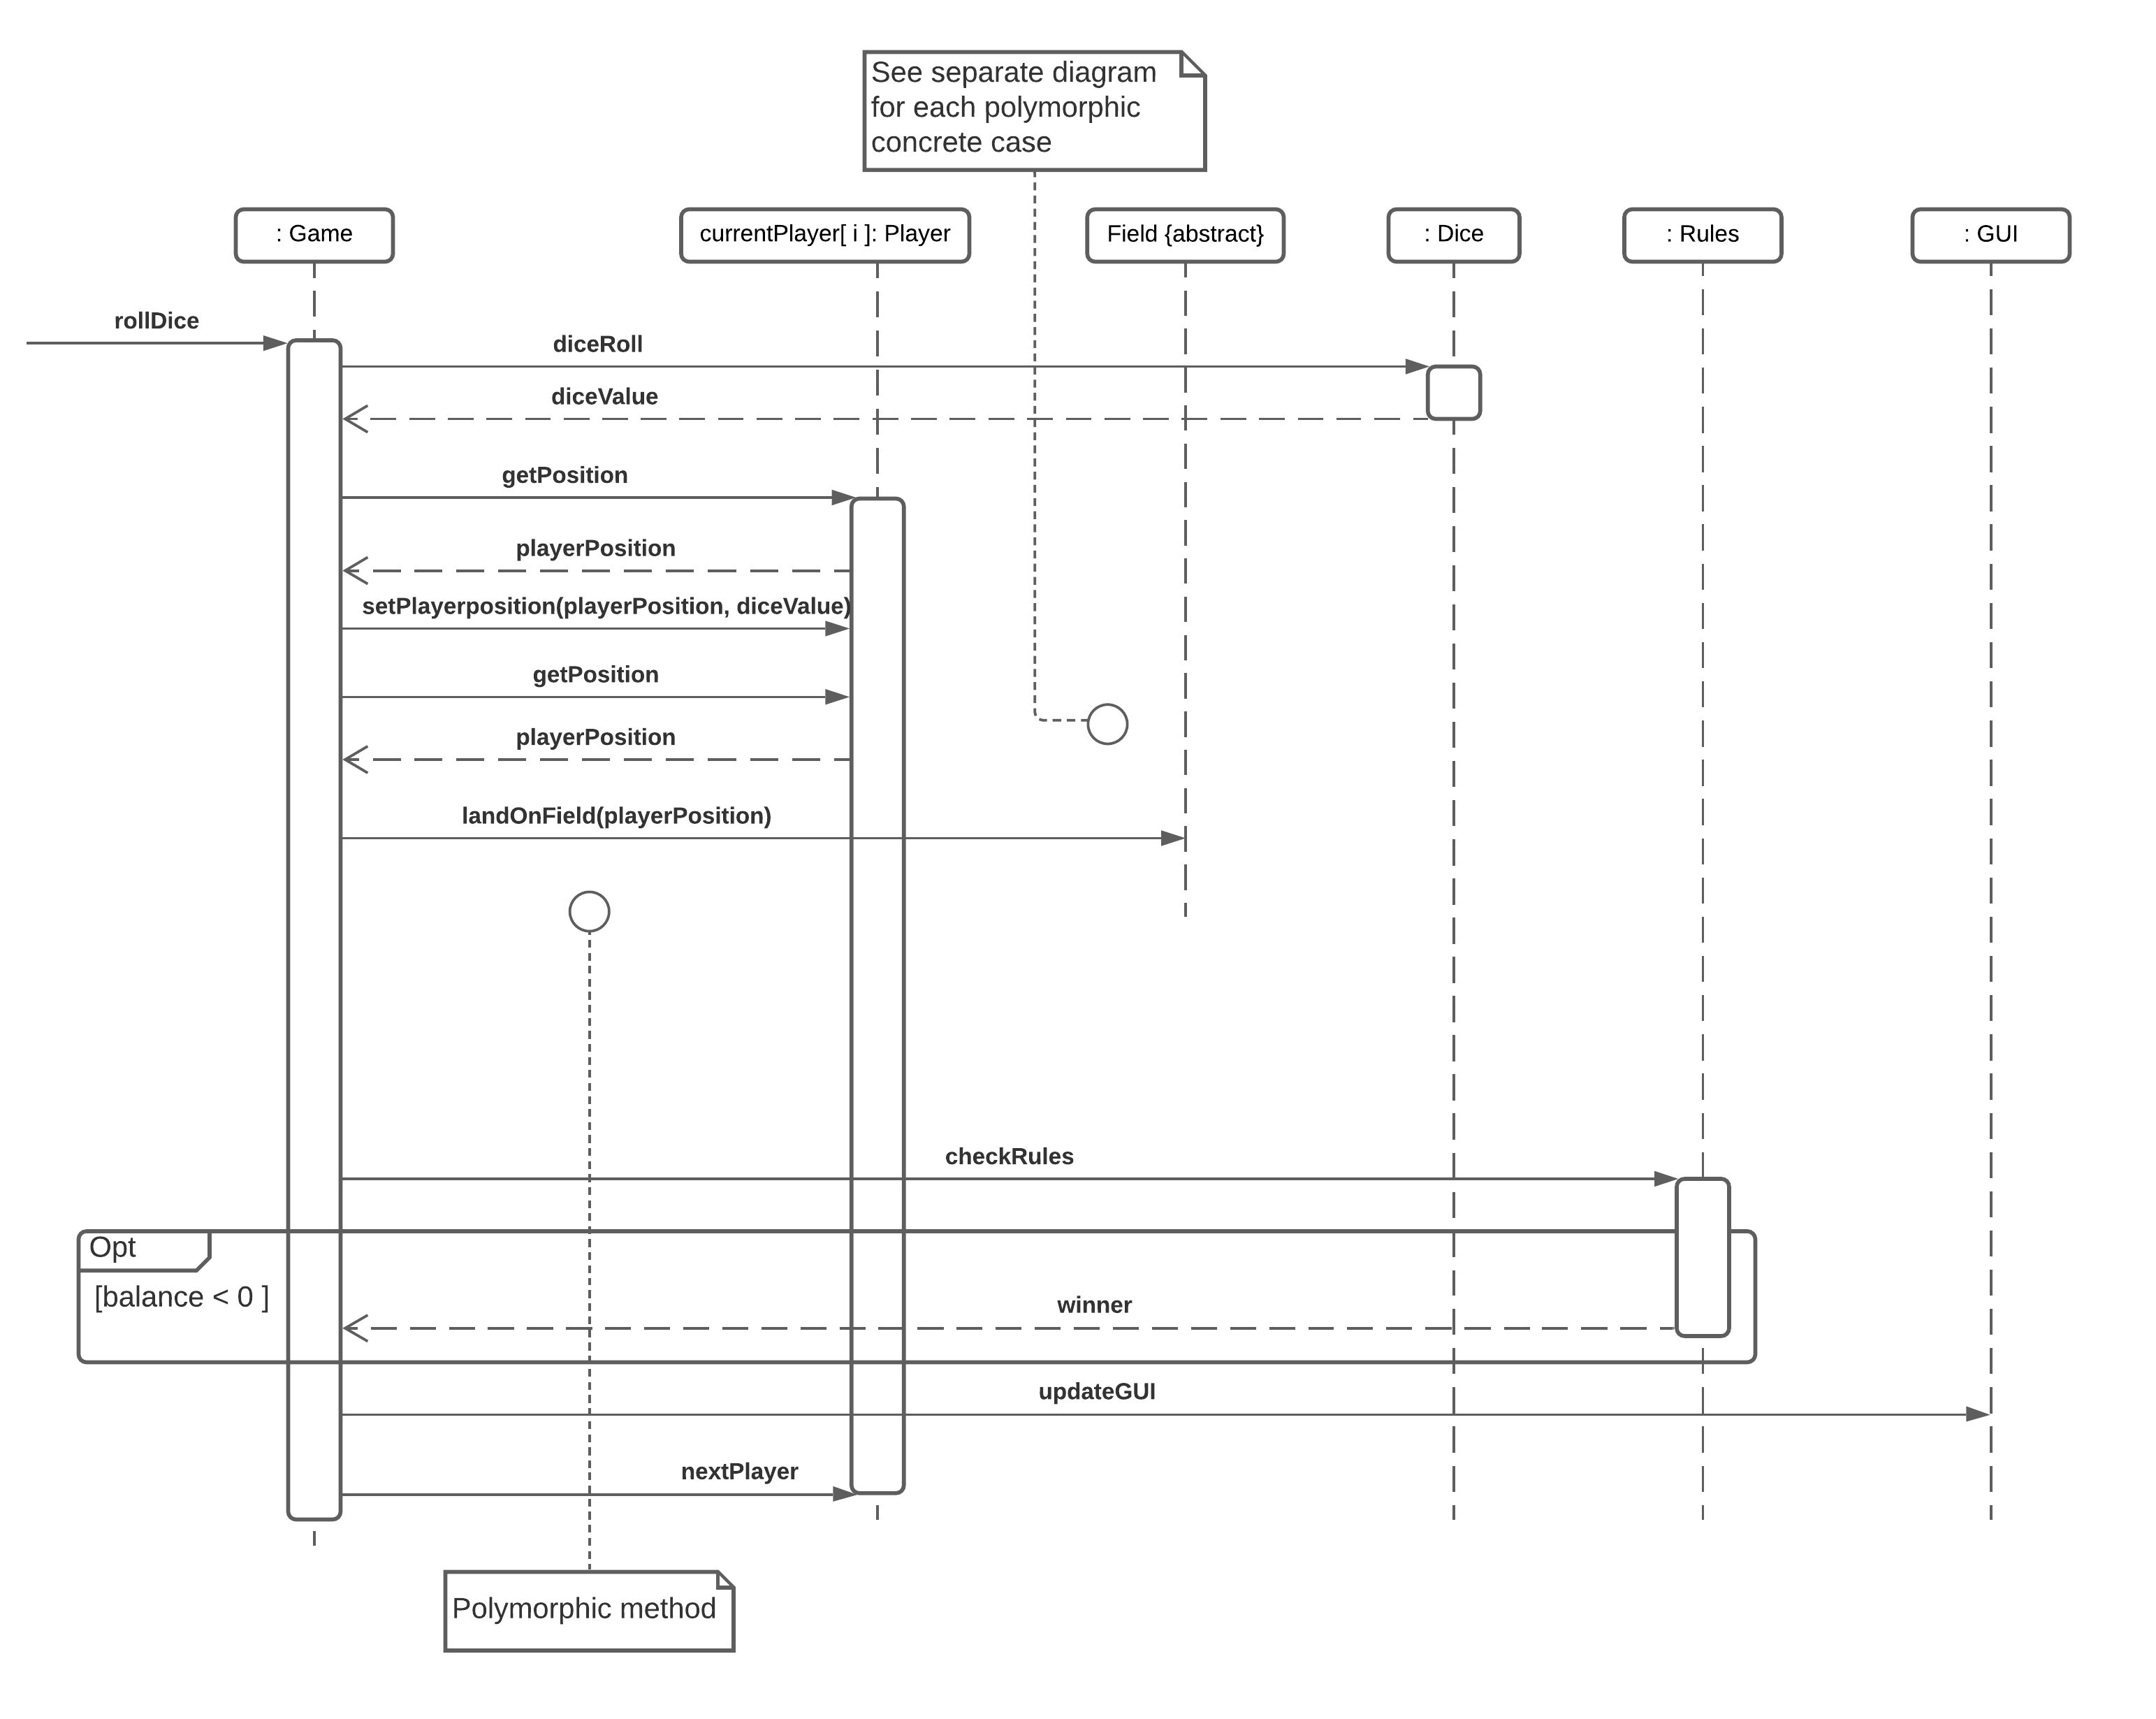
\includegraphics[width=1\textwidth]{Report/figures/Sekvensdiagram1.png}~\\[0cm]
Figur 5.1.1. Sekvensdiagram over rollDice som use-case.

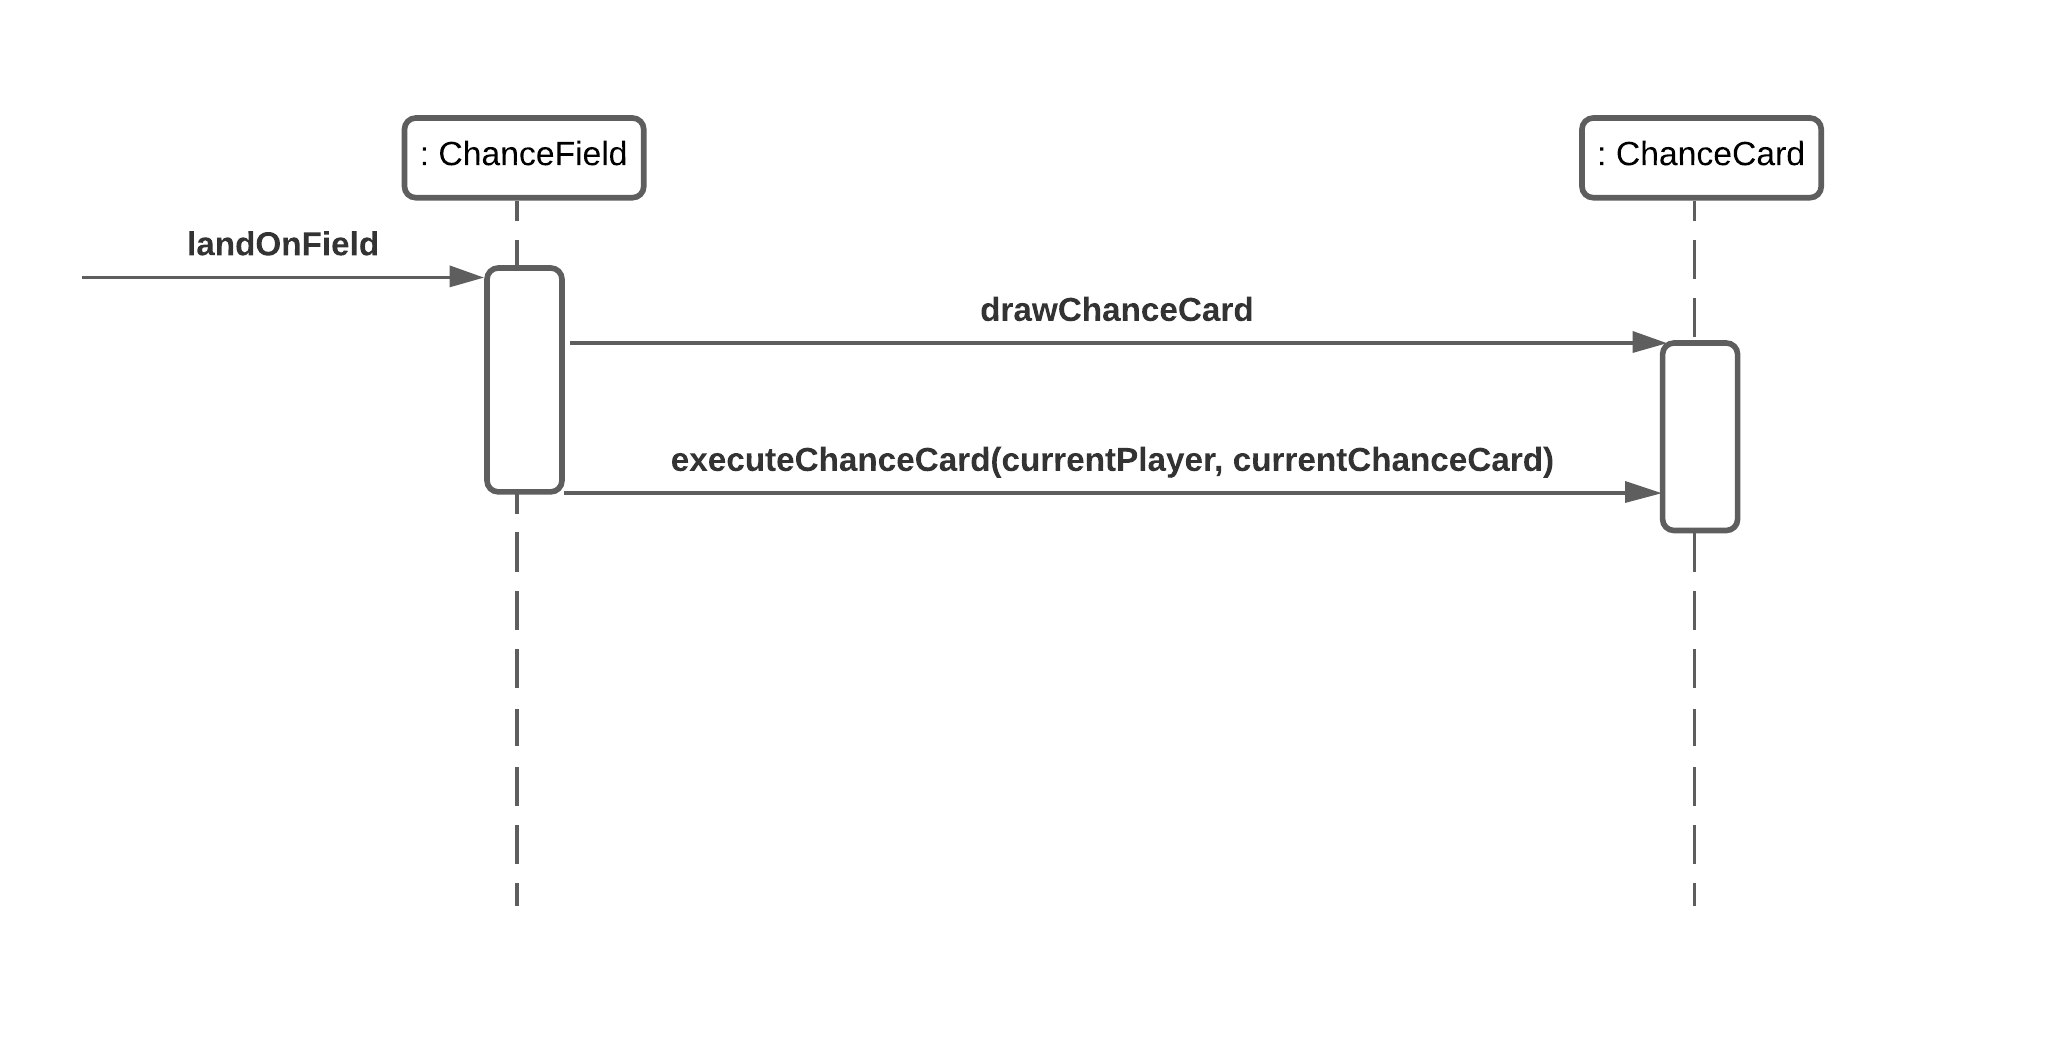
\includegraphics[width=0.9\textwidth]{Report/figures/Sekvensdiagram_ChanceField.png}~\\[0cm]
Figur 5.1.2. Sekvensdiagram over polymorphism af metoden landOnField for ChanceField.


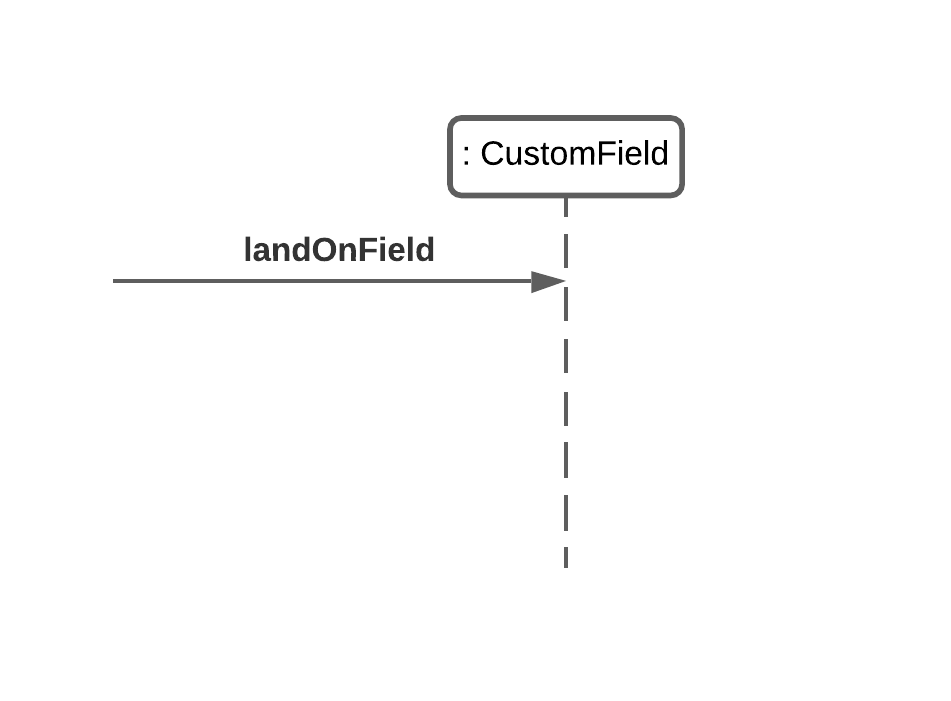
\includegraphics[width=0.9\textwidth]{Report/figures/Sekvensdiagram_CustomField.png}~\\[0cm]
Figur 5.1.3. Sekvensdiagram over polymorphism af metoden landOnField for CustomField.


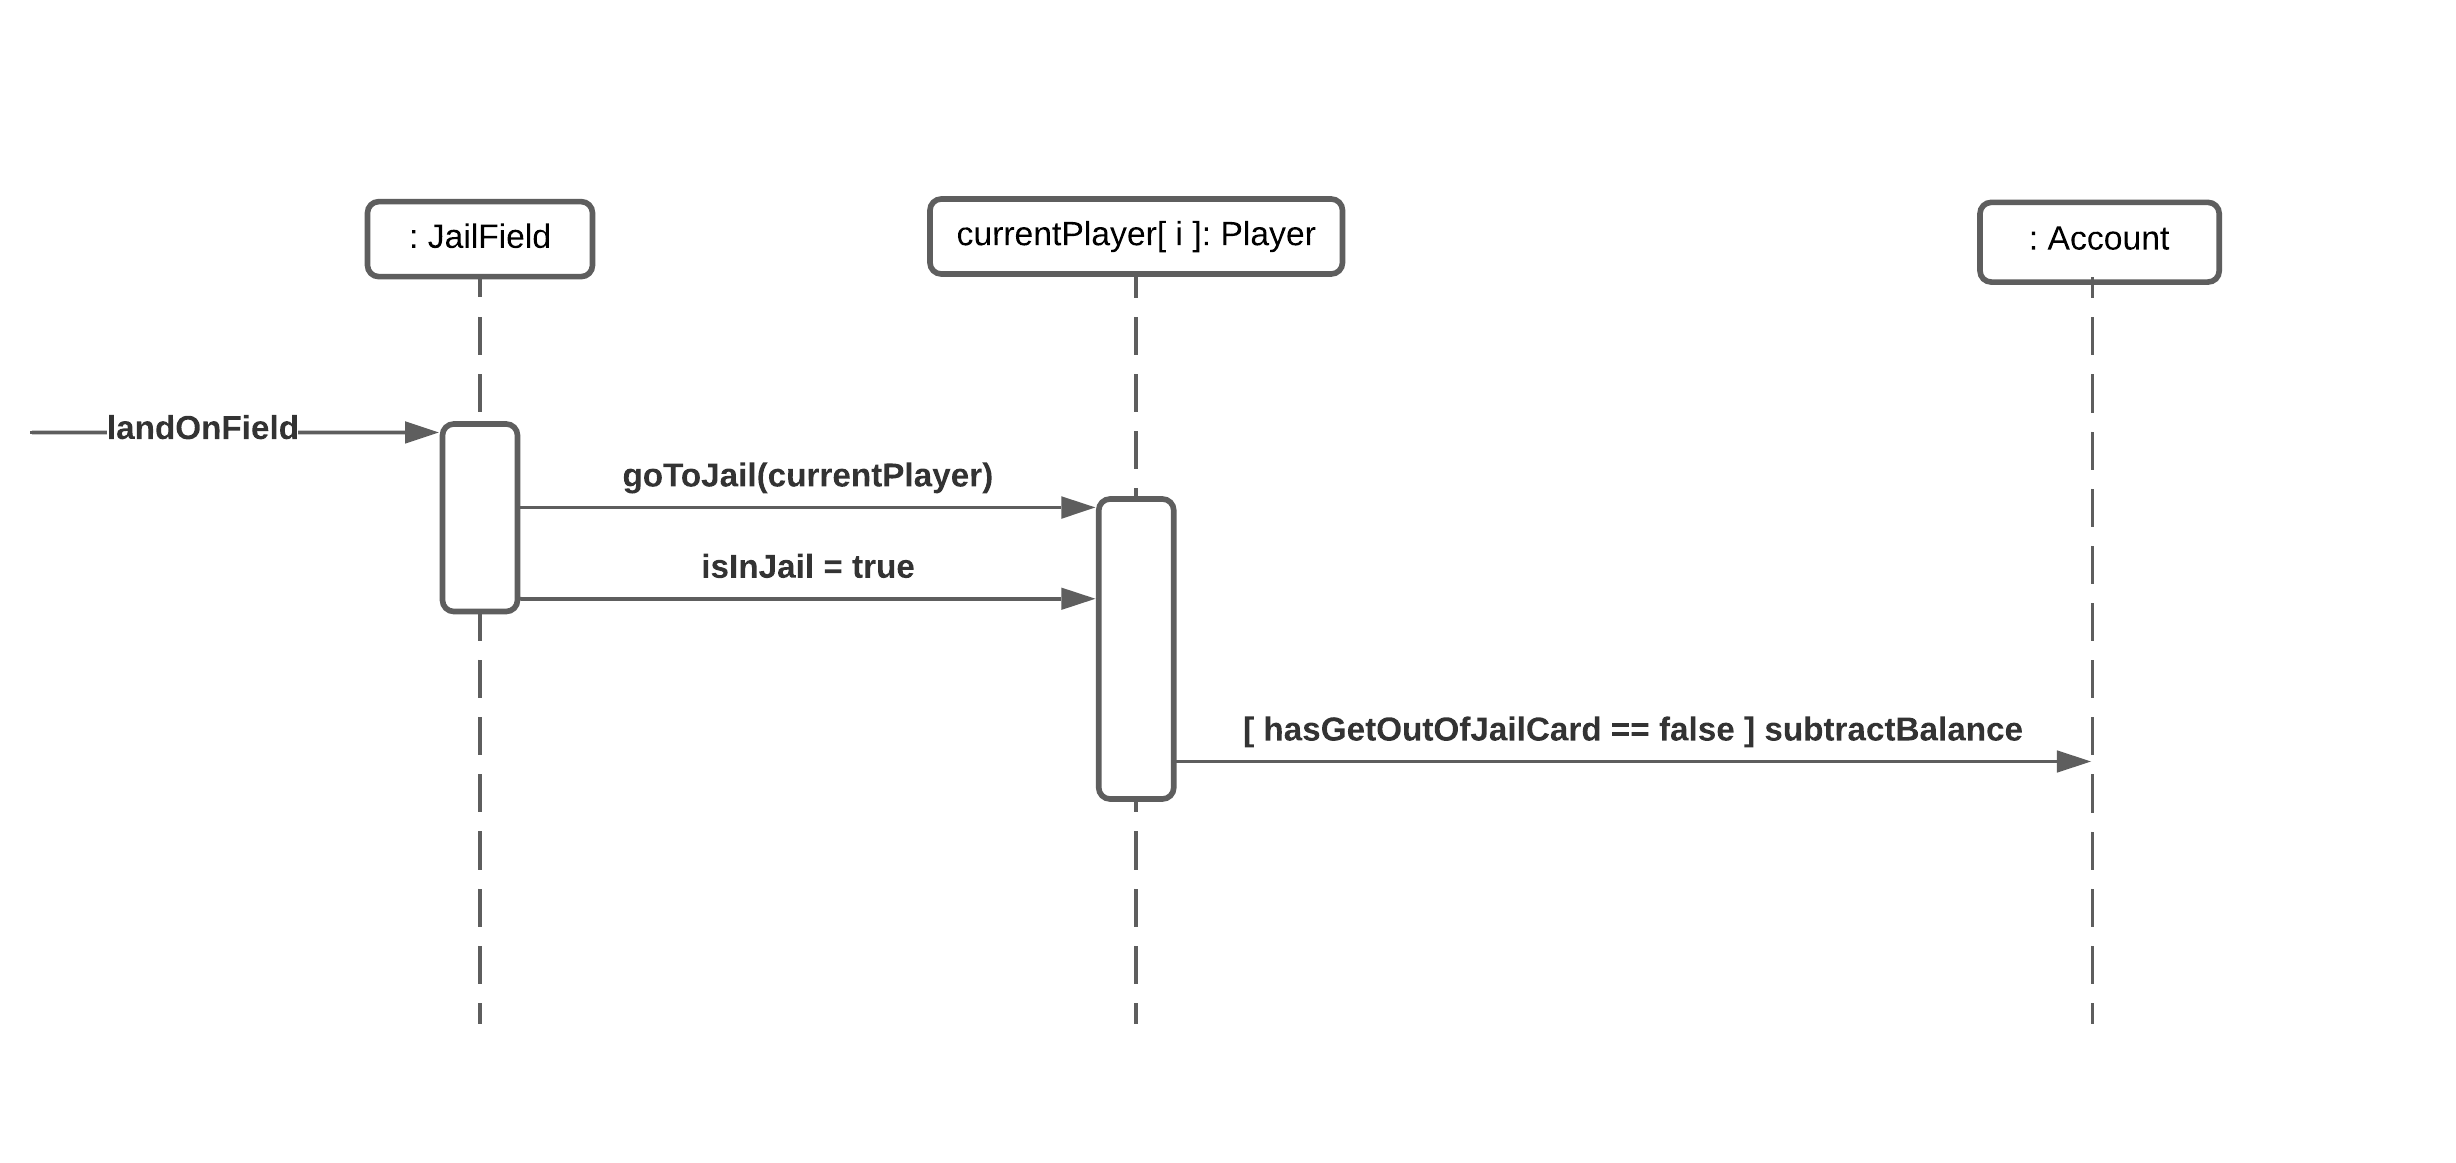
\includegraphics[width=0.9\textwidth]{Report/figures/Sekvensdiagram_JailField.png}~\\[0cm]
Figur 5.1.4. Sekvensdiagram over polymorphism af metoden landOnField for JailField.


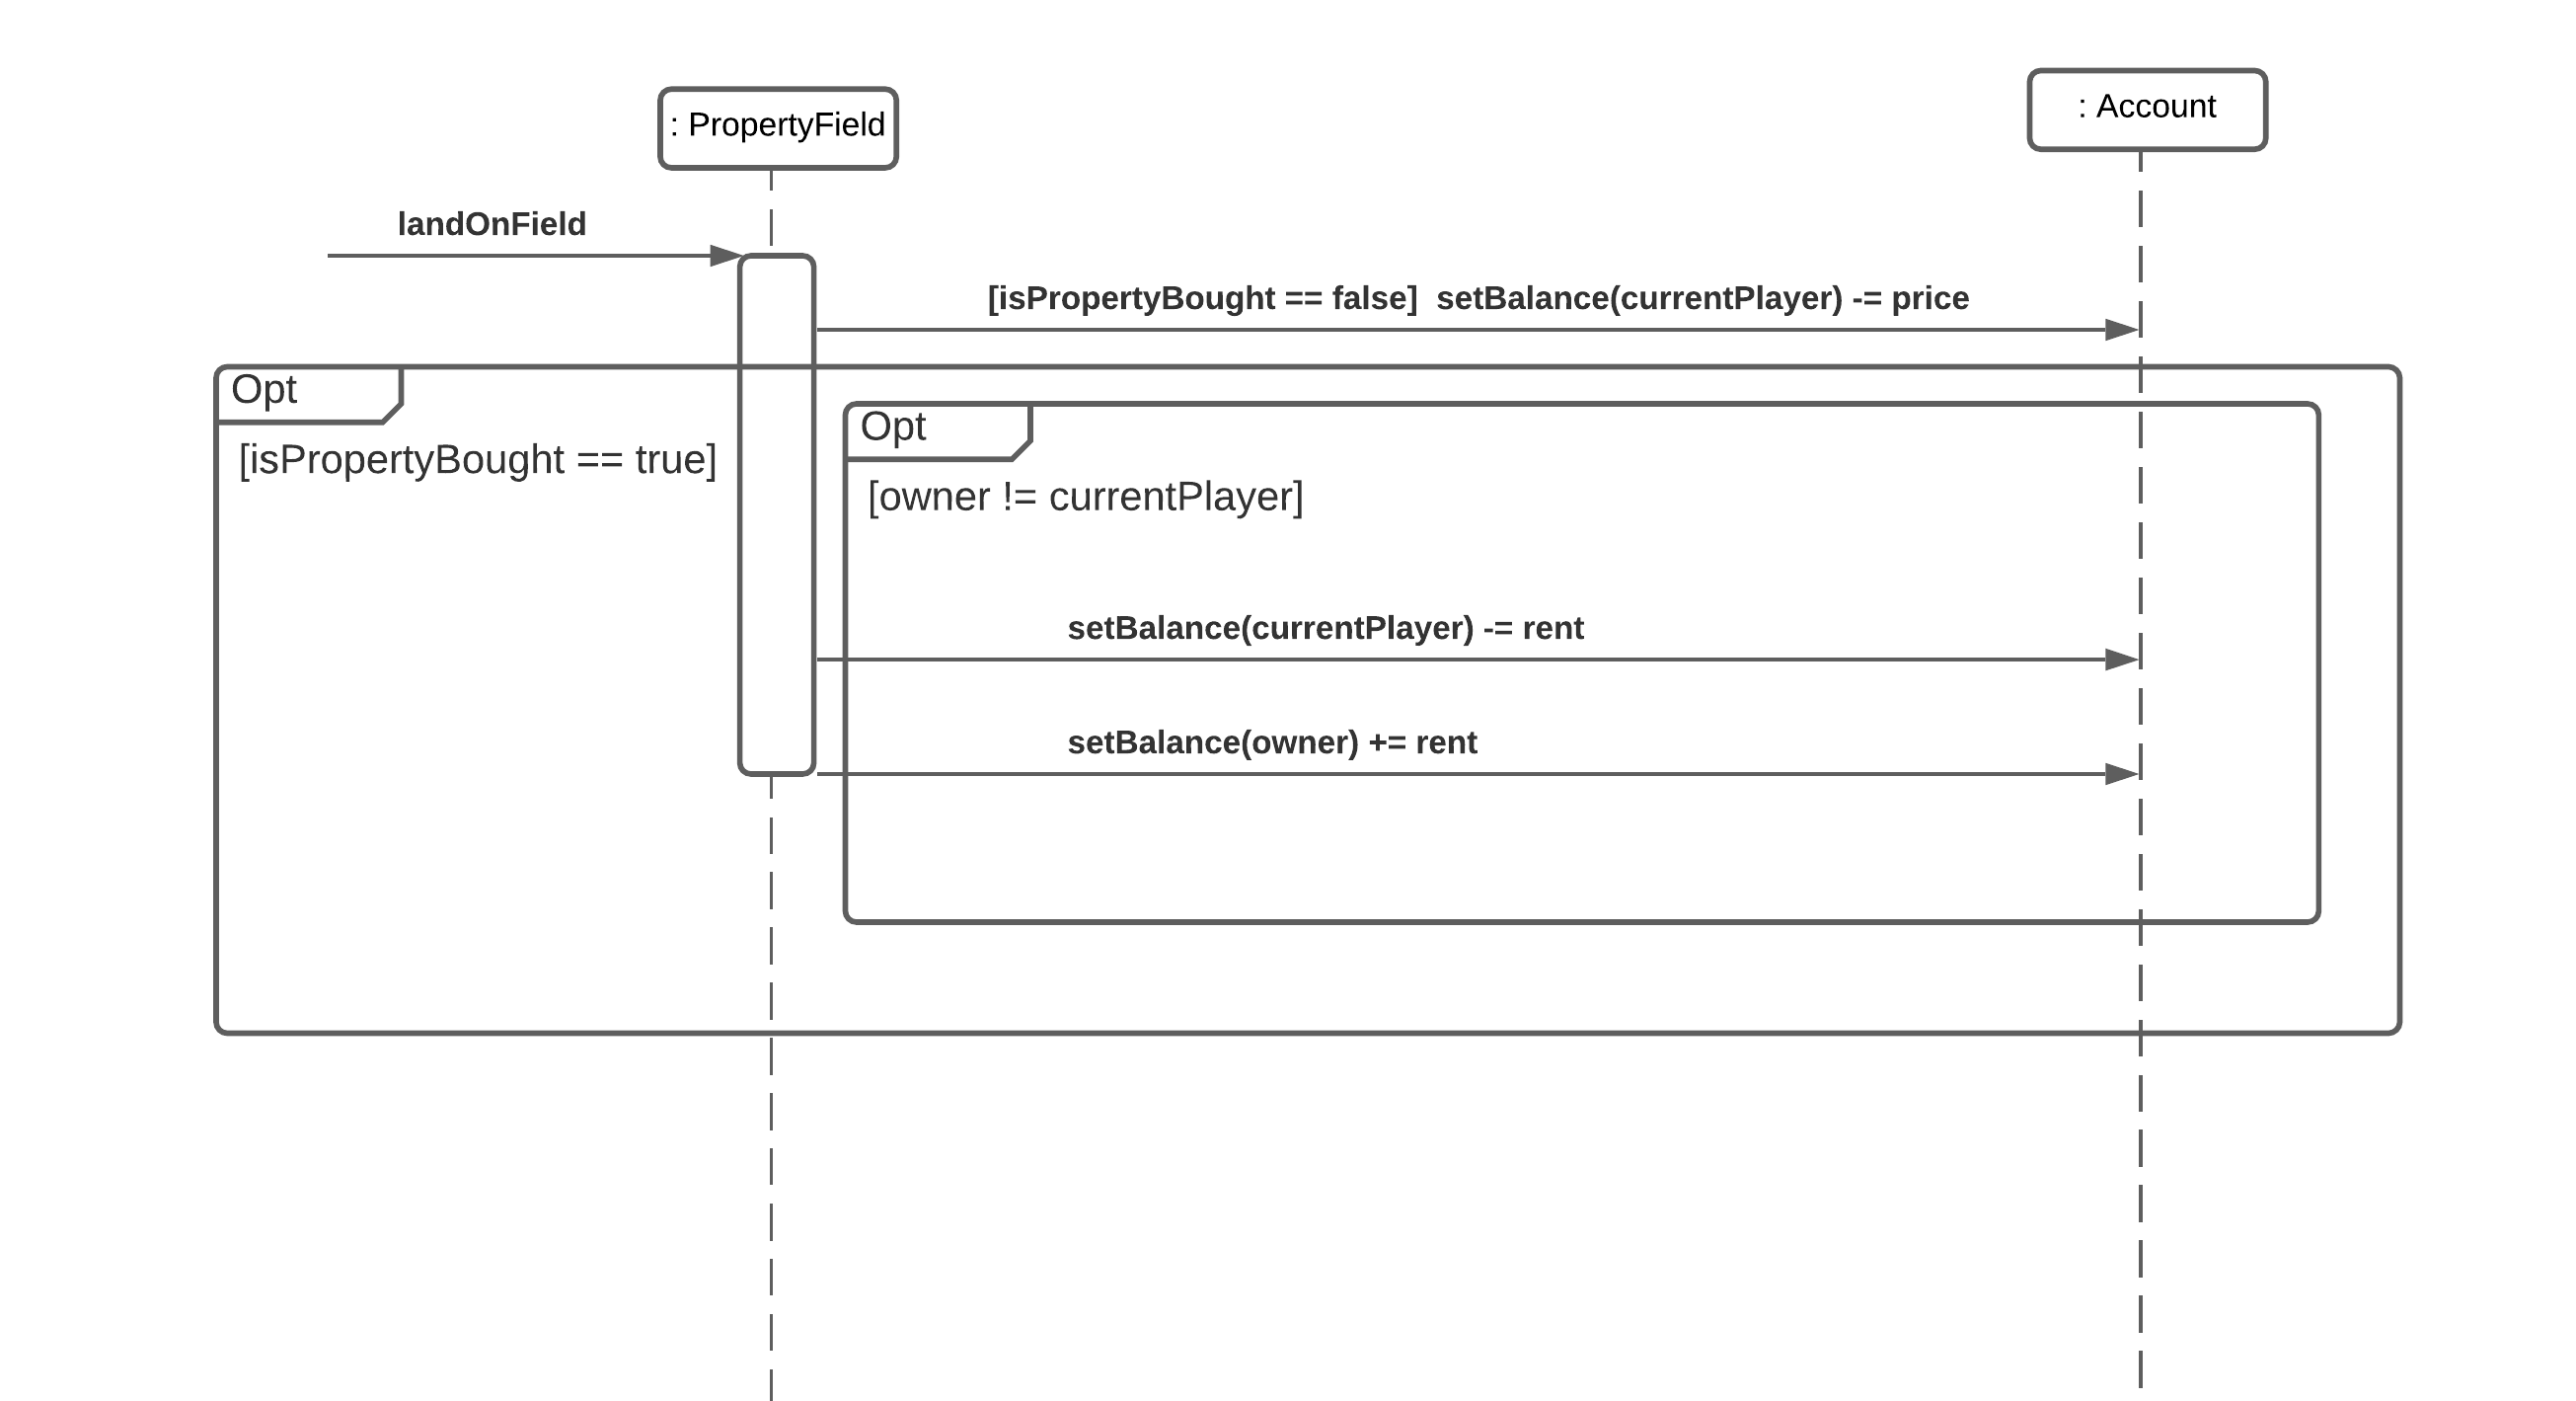
\includegraphics[width=0.9\textwidth]{Report/figures/Sekvensdiagram_PropertyField.png}~\\[0cm]
Figur 5.1.5. Sekvensdiagram over polymorphism af metoden landOnField for PropertyField.


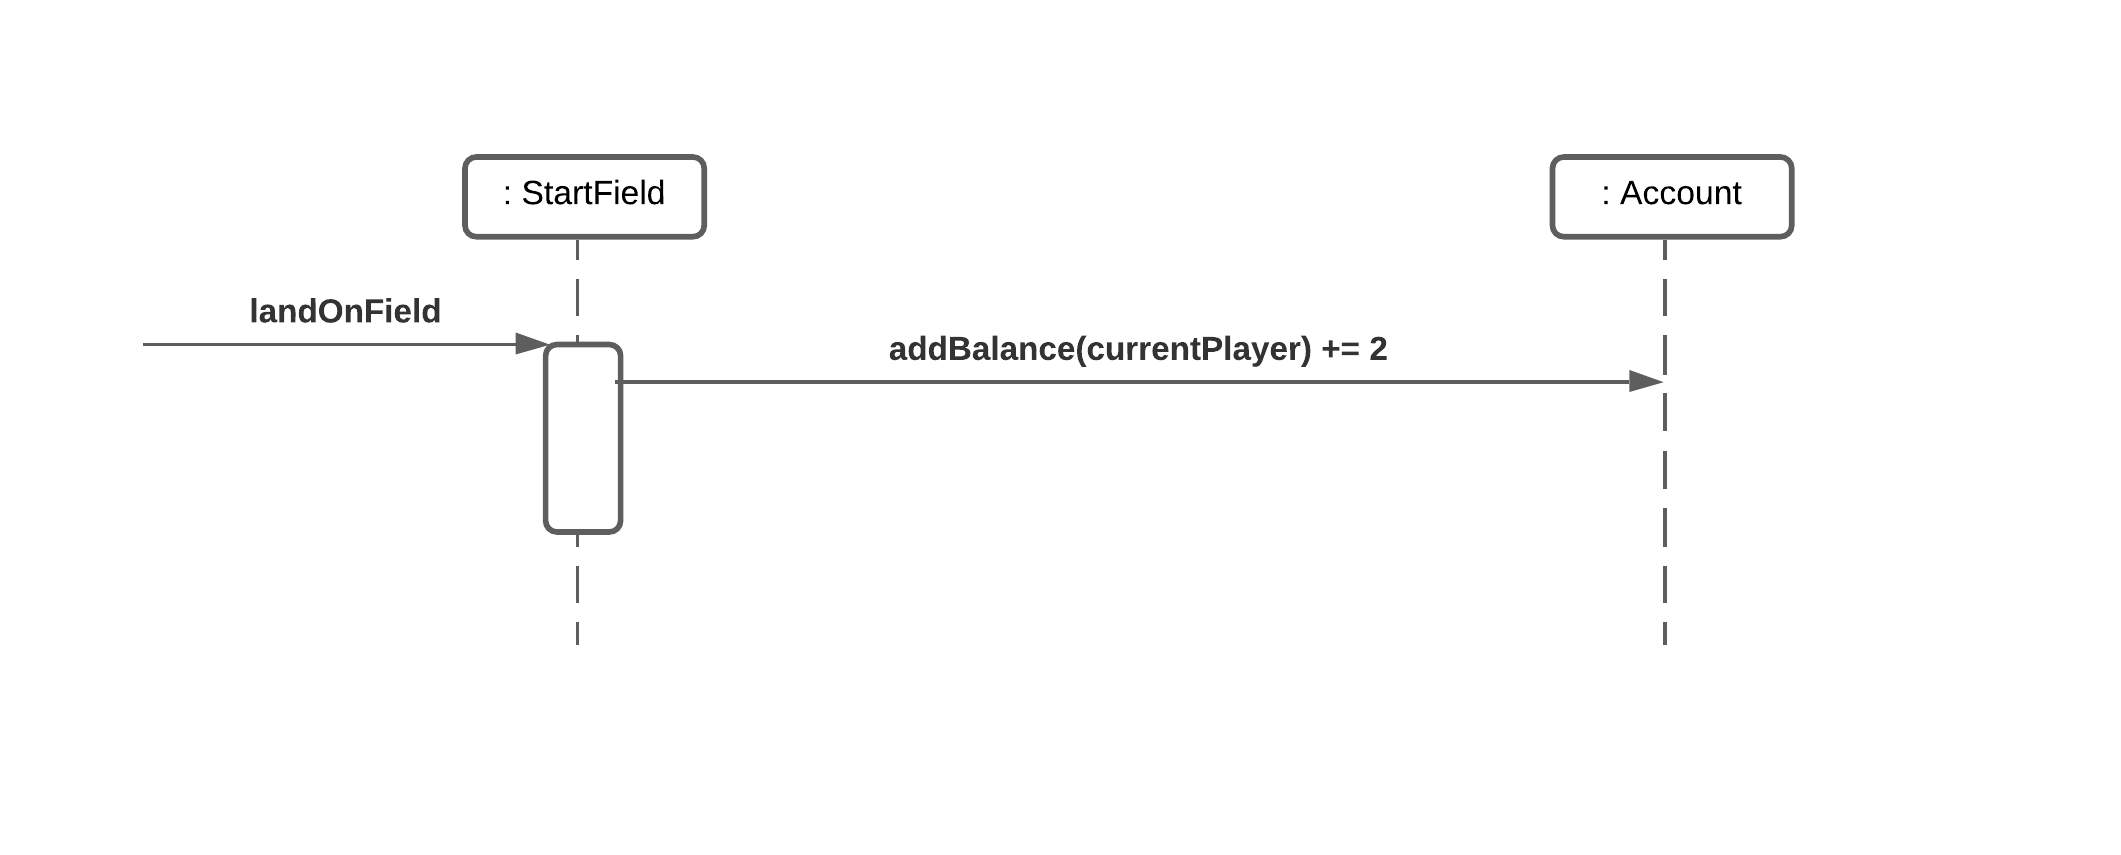
\includegraphics[width=0.9\textwidth]{Report/figures/Sekvensdiagram_StartField.png}~\\[0cm]
Figur 5.1.6. StartField over polymorphism af metoden landOnField for ChanceField.
\subsection{Designmønster GRASP}
I dette afsnit beskriver vi kort, hvordan vores design har overholdt GRASP principper. Her refereres der til designklassediagrammet (se figur 5.2.1) uden at danne en fyldestgørende beskrivelse af dette diagram. For en fyldestgørende beskrivelse af designdiagrammet, se afsnit 5.3.
\paragraph*{Creator:} I designklassediagrammet ses det, at vi har opdelt ansvaret for creators, således at der findes fire controllers, der har ansvaret for at instantiere objekter af klasser forskellige klasser: ChanceCardController, FieldController, PlayerController, GUIController og DiceController.

\paragraph*{Controller:}
Her har vi indført de tidligere nævnte controllers, der har forskellige ansvar for at bearbejde handlinger og metoder i systemet. Controllers bearbejder altså den klasse, de er ansvarlige for og videresender denne information i systemet. Herudover kan Menu også anses som en controller, der styrer brugerinput inden spillet er sat igang.

\paragraph*{Low Coupling:}
I vores designmønster har vi stræbt efter low coupling. Det vil sige, at vores klasser har få relationer til hinanden, da der veldefinerede ansvarsområder. F.eks. ses det, at ChanceCard ikke har en relation til andet end ChanceCardController, da dette objekt jo netop tager ansvaret for metodernei klassen.

\paragraph*{High Cohesion:}
Vi har sørget for at overholder principper om high cohesion ved kun at definere ansvar for klasser, hvor det er relevant. F.eks. ses det, at vi har opdelt Player i Player og Account, som gør, at hver klasse har mere præcise definerede ansvarsområder.

\paragraph*{Polymorphism:}
Vores brug af polymorphism ses specifikt ved Field klassen, der nedarves af fem forskellige klasser. Her er metoden landOnField polymorfisk, da udførslen er varierer mellem de forskellige nedarvede klasser.

\paragraph*{Information Expert:}
Det ses, at vi stræber efter, at klasser kun udfører handlinger, som de har nok information til at udføre. F.eks. udfører DiceController kun handlinger, der vedrører Dice - se metodern diceRoll() og diceValue().

\paragraph*{Protected Variation:}
For at overholde protected variation gør vi brug af dataindkapsling for variable og nedarvning for Field klassen. Dette gør, at de forskellige delelementer i systemet er "beskyttede" fra ændringer i andre delelementer.

\subsection{Designklassediagram}
Vores designklassediagram er en udbyggelse af domænemodellen og sekvensdiagrammet (se figur 5.2.1). Vi har altså en Gameloop klasse, der styrer hele spillet og danner nye objekter for controllers, Menu og Rules. Her ses det, at hver controller har et veldefineret ansvarsområde. F.eks. er FieldController ansvarlig for Field klassen. For Player klassen ses det, at Account er en komposition. Dette er dels fordi account ikke eksisterer uden en Player.
\begin{center}
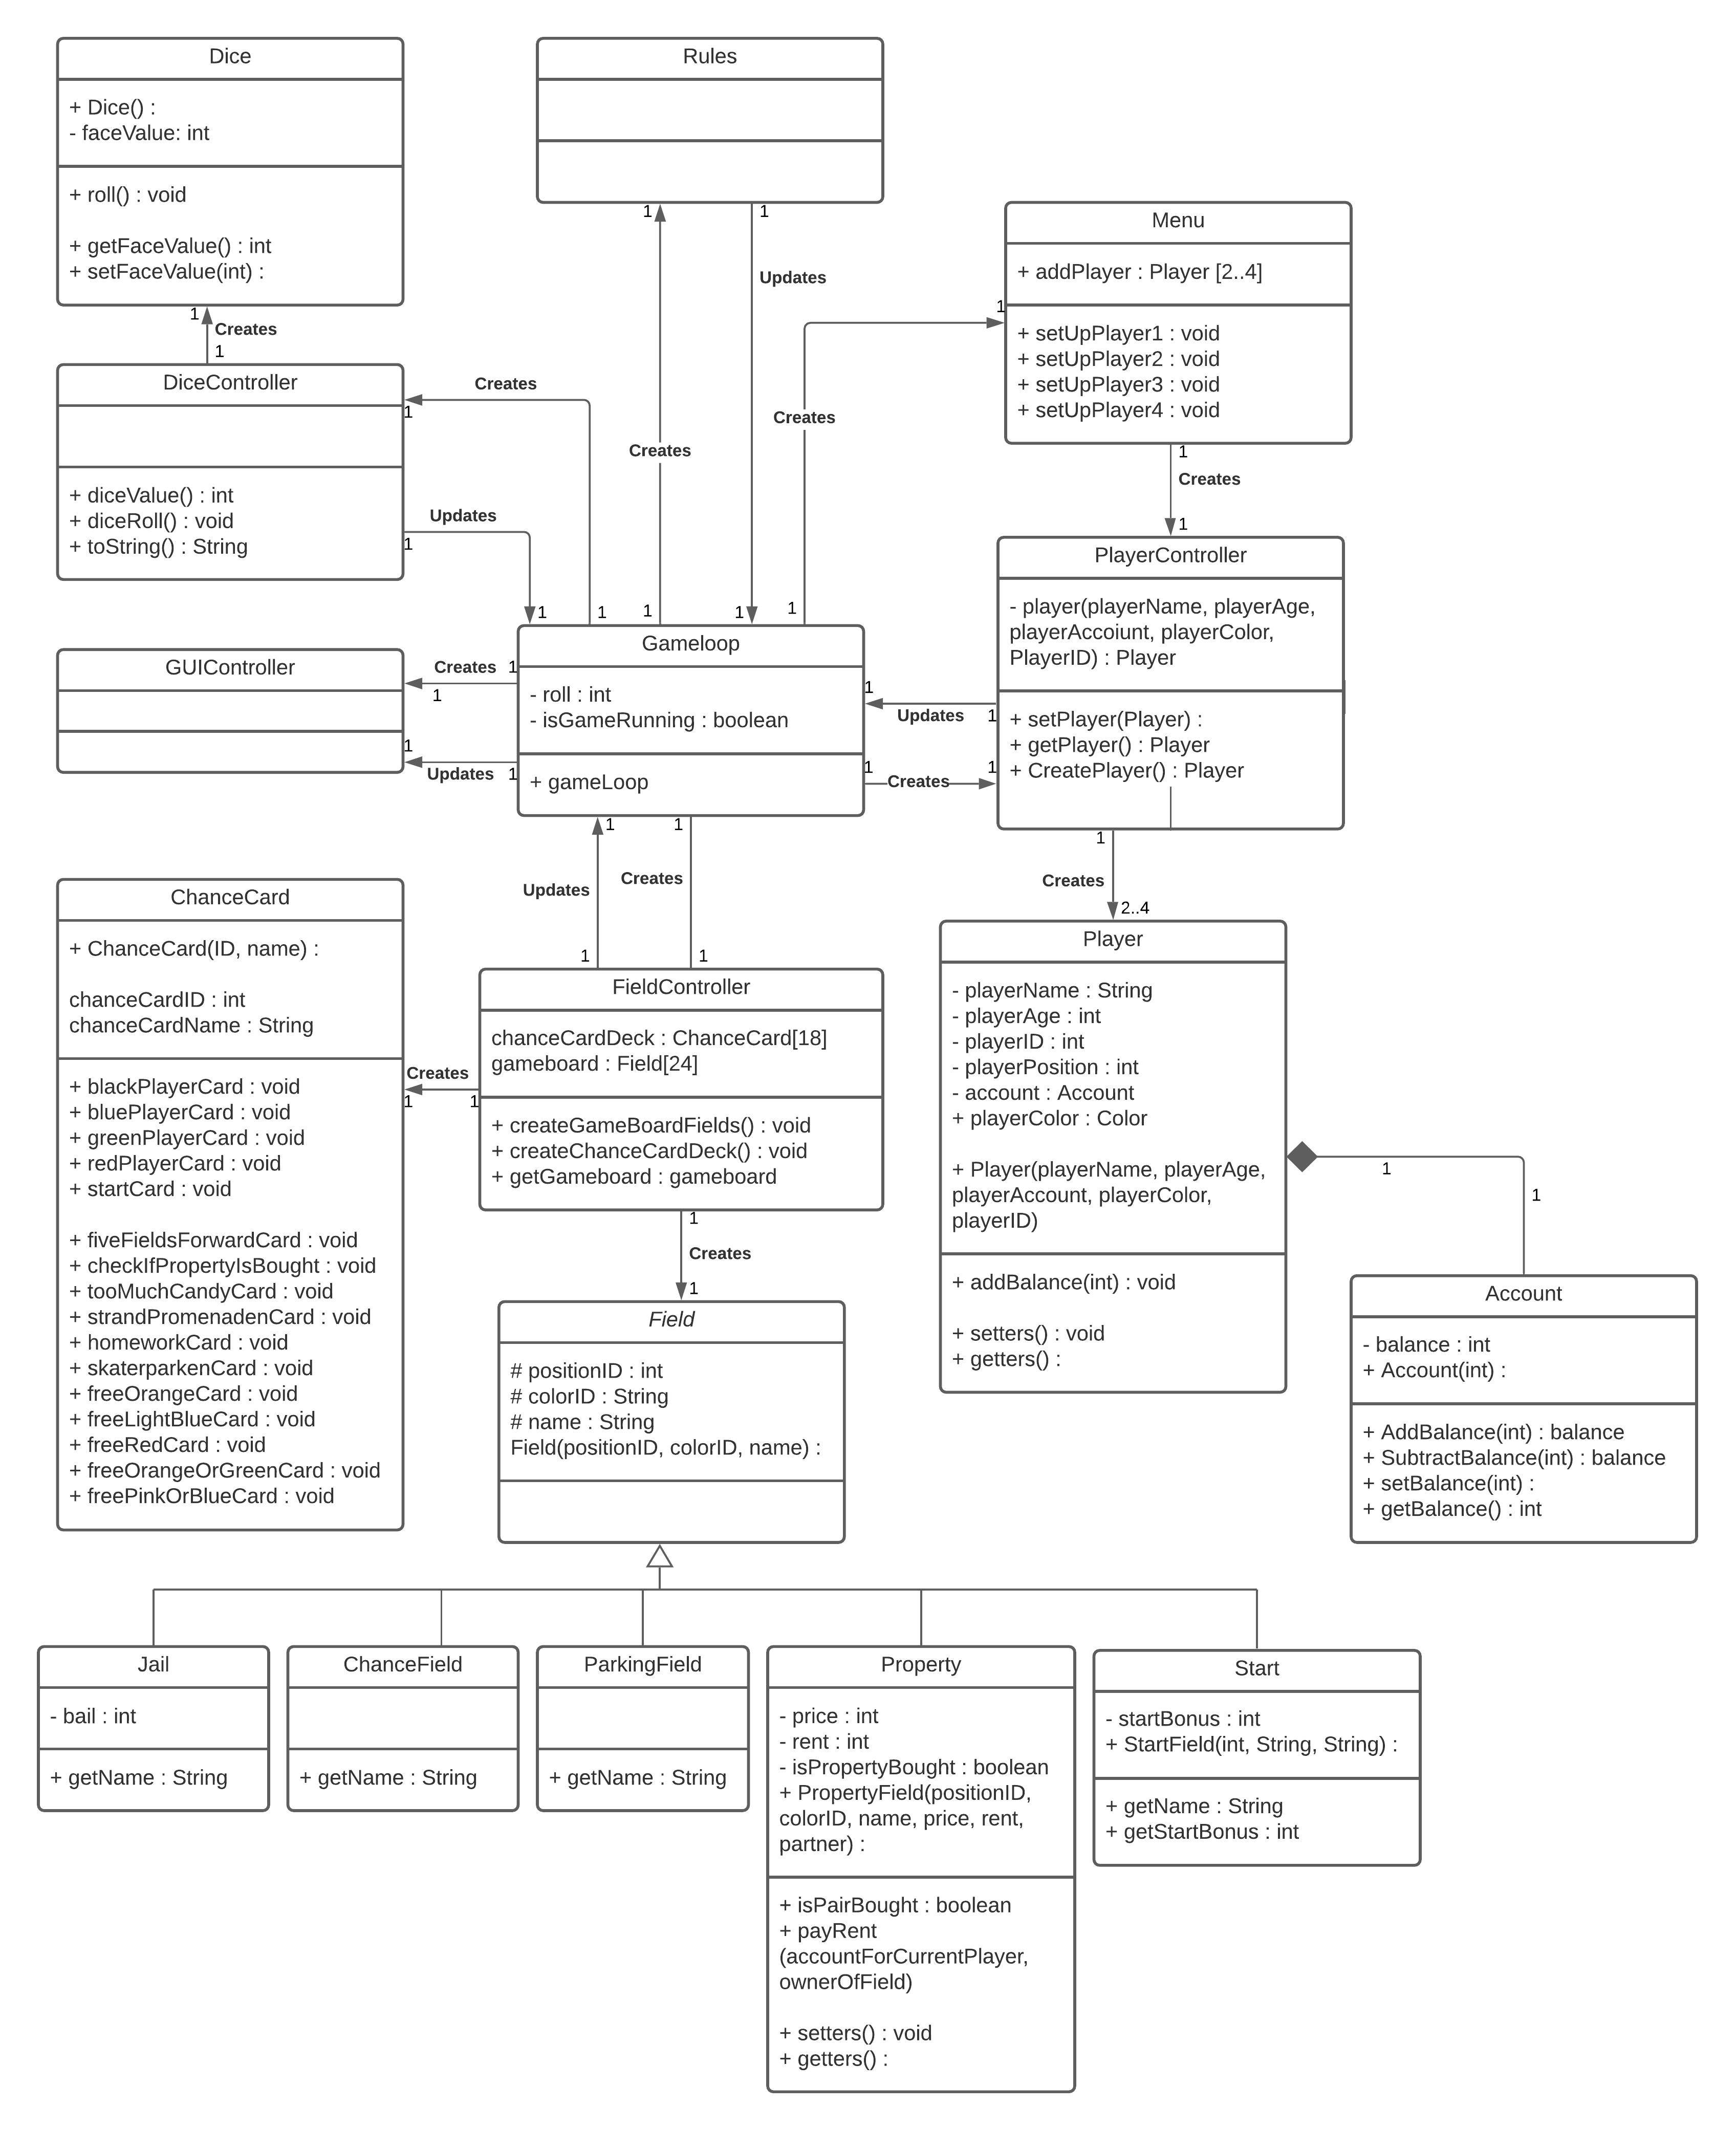
\includegraphics[width=1\textwidth]{Report/figures/Class Diagram.png}~\\[0cm]
\end{center}
Figur 5.2.1. Designklassediagram over Monopoly Junior spillet.
\end{flushleft}